\section{Introduction}
JavaScript is one of the most widely used programming languages not only for client-side
but also for server-side programming~\cite{nodejs, meanjs}
and even for small embedded systems~\cite{espruino, tessel2}.
It is the top-ranked language used in active GitHub
repositories\footnote{https://githut.info/}, and \#7 in the TIOBE
Programming Community index\footnote{https://www.tiobe.com/tiobe-index/}.
According to W3Techs\footnote{https://w3techs.com/technologies/details/cp-javascript/all/all},
95.2\% of websites use JavaScript as their client-side programming language.

Despite its popularity, JavaScript developers often suffer from its intricate semantics,
which may cause unexpected behavior.  For example, calling the following JavaScript
function seems to always return \( \code{false} \):
\begin{lstlisting}[style=myJSstyle]
    function f(x) { return x == !x; }
\end{lstlisting}
Unfortunately, it returns \( \code{true} \) when its argument is an empty array
\( \code{[]} \).  To correctly understand and reason about such complex
behavior, the formal semantics of JavaScript is necessary.

\begin{figure}
  \centering
  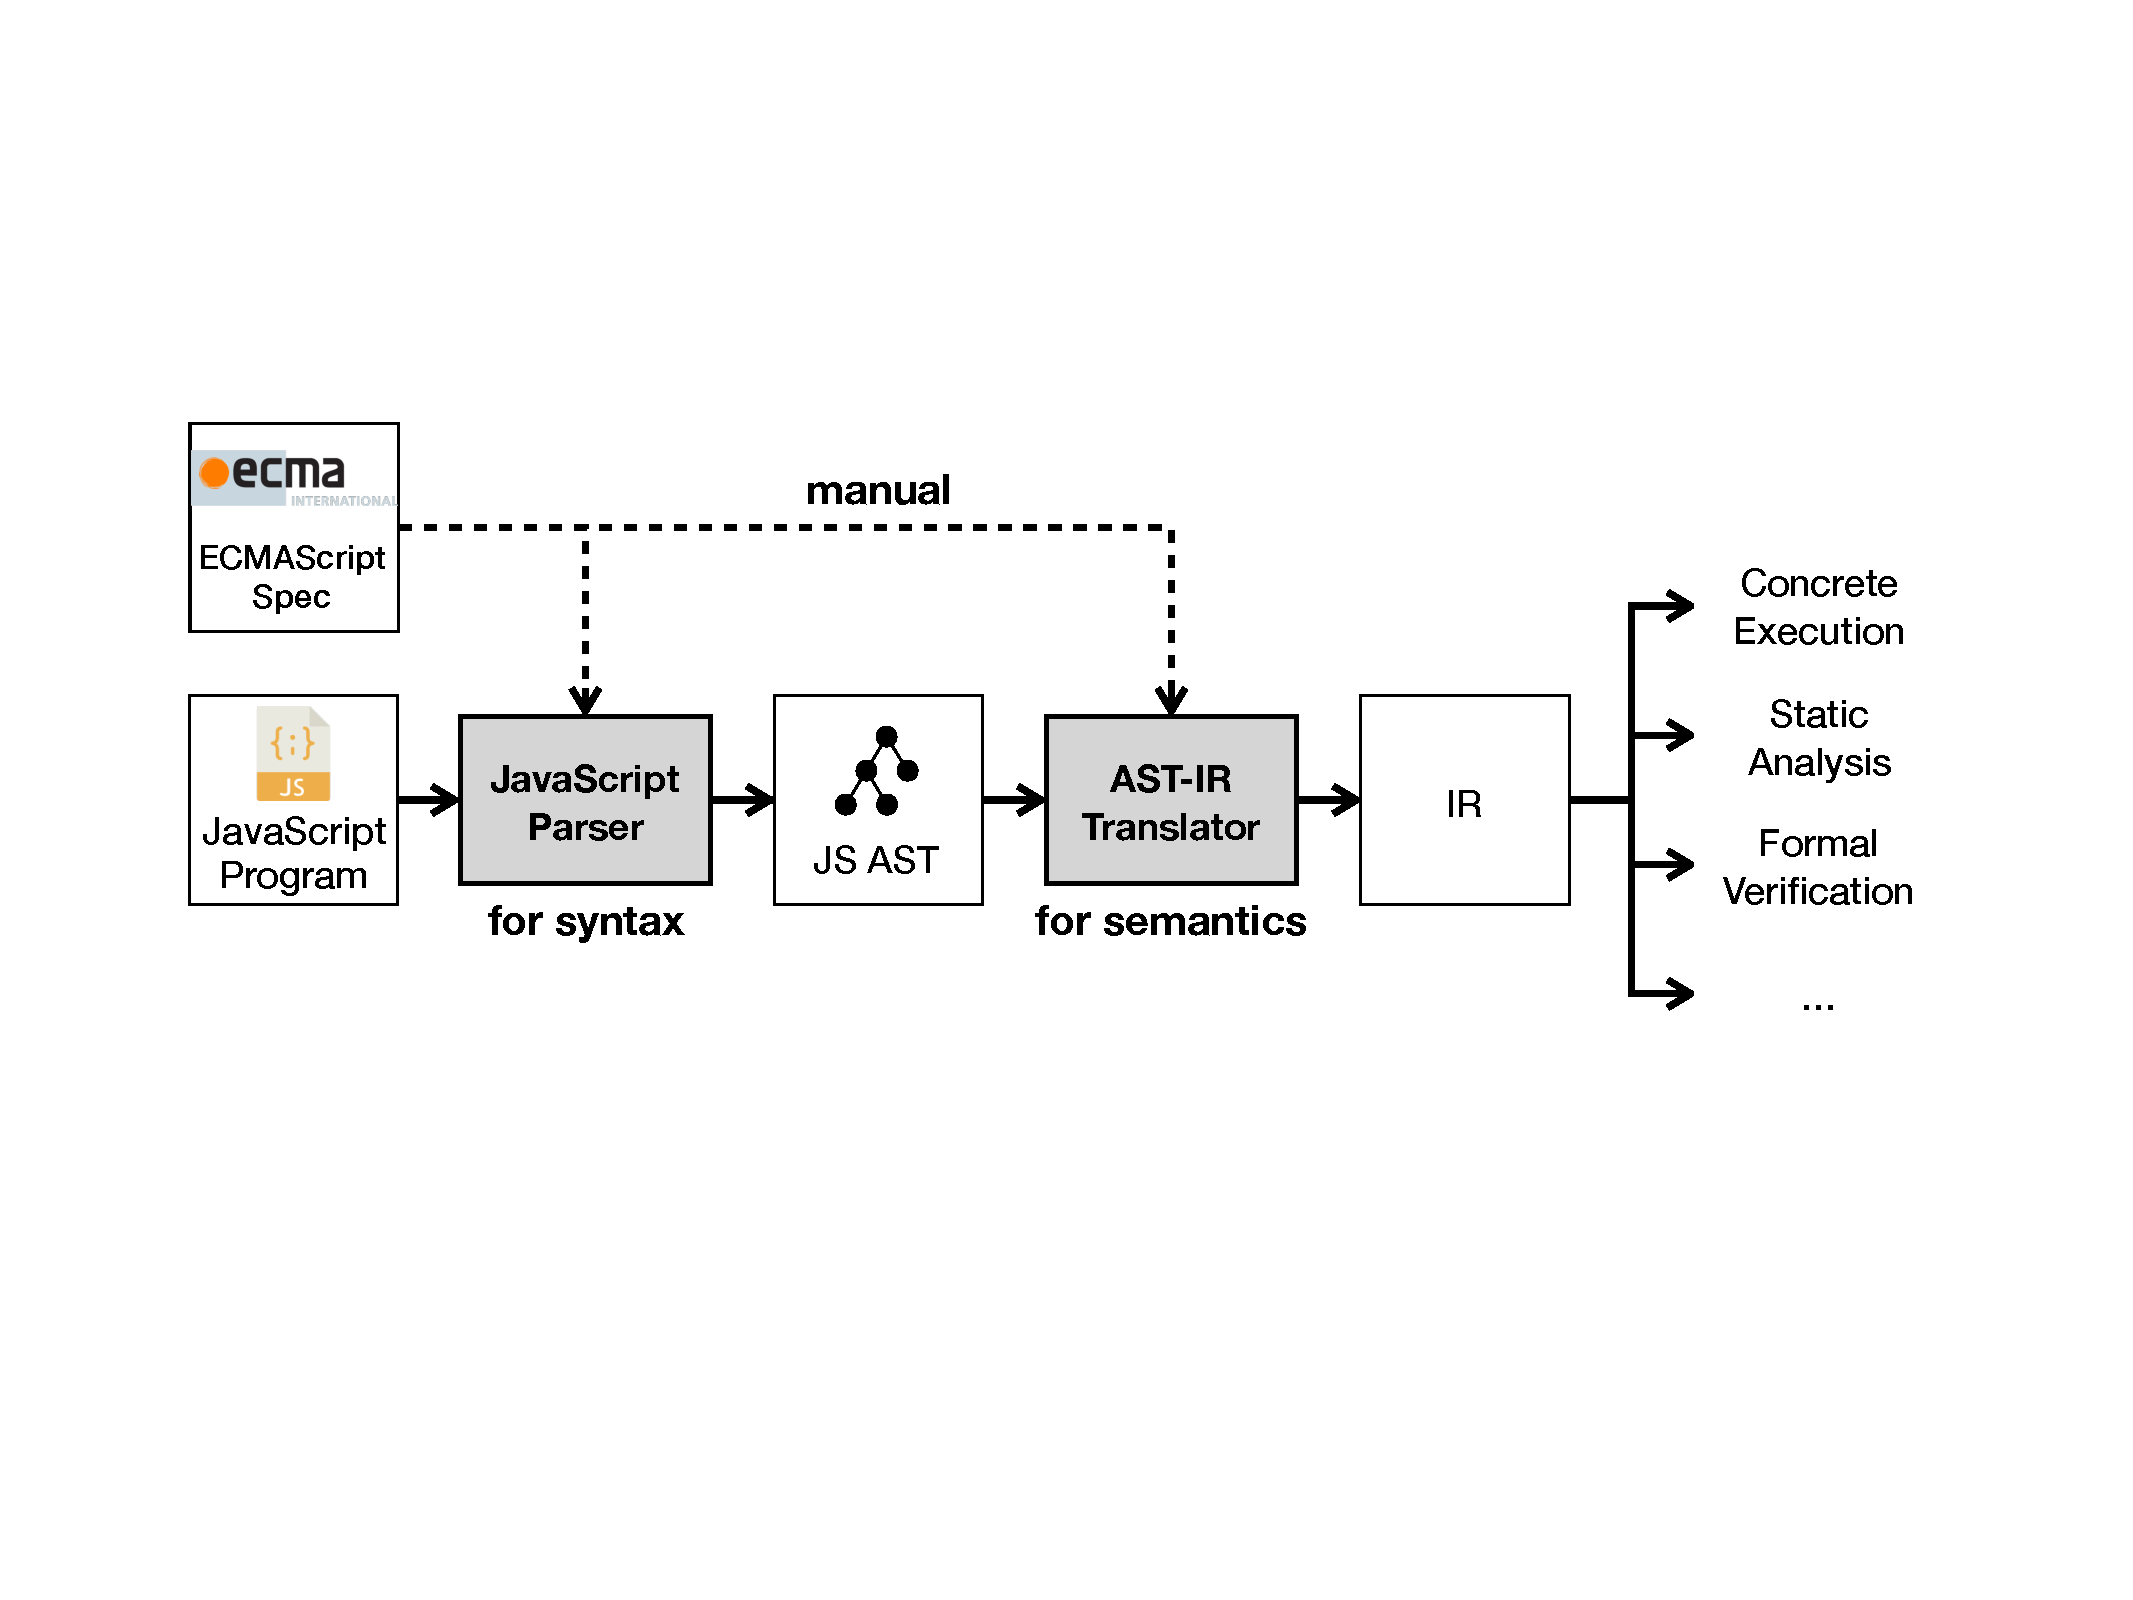
\includegraphics[width=0.48\textwidth]{img/existing.pdf}
\vspace*{-2em}
  \caption{Existing approaches: Manually implemented parsers and AST-IR
  translators for IR-based semantics of JavaScript programs}
  \label{fig:existing}
\vspace*{-1em}
\end{figure}

Researchers have defined various JavaScript formal
semantics~\cite{aplas08,lambdajs,kjs,javert} suitable for static
analysis~\cite{jsai,tajs,wala,safe} and formal verification~\cite{javert} by
referring to ECMAScript specification.  ECMAScript specification officially
describes JavaScript syntax using a variant of extended BNF notation, and its
semantics using abstract algorithms written in English in a clearly and
structured manner.  As illustrated in Figure~\ref{fig:existing}, they built
parsers that constructs Abstract Syntax Trees (ASTs) of given JavaScript
programs, and AST-IR translators to convert ASTs to their own Intermediate
Representations (IRs). This approach helps researchers focus on IRs without
worrying about diverse and enormous features of JavaScript in developing new
techniques for program analysis and formal verification.  We dub such
methodology that manipulates language semantics by translating given programs to
IRs \textit{IR-based semantics extraction}.

However, to the best of our knowledge, all existing approaches to JavaScript
IR-based semantics extraction \textit{manually} build parsers and translators.
The manual approach is tedious, labor-intensive, and error-prone.  For example,
KJS~\cite{kjs} is one of formal semantics for traditional JavaScript described
in ECMAScript 5.1 specification~\cite{ecma5} (ES5.1, 2011) and it is defined on top of \(
\kframework \), which is a framework for defining language semantics.  According
to an author of KJS, it took \textit{four months} to implement AST-IR translator
for 1,370 lines out of 2,932 lines in 368 abstract algorithms. However, modern
JavaScript becomes much more massive than traditional one and the most recent
version of ECMAScript specification (ES10, 2019) has 1,731 abstract algorithms
consisting of 10,068 lines.  It means that it is not scalable to build AST-IR
translator for modern JavaScript.  Thus, most of JavaScript formal semantics
targets for ES5.1 and no formal semantics deals with modern JavaScript features
such as lexical binding via \( \code{let} \), the spread \( \code{...} \)
operator, classes, the \( \code{for-of} \) operator, the \( \code{async} \)
functions, and generators.

Moreover, JavaScript syntax and semantics is annually updated.  Until ECMAScript
5.1 specification, JavaScript is quite stable language because the specification
has been rarely updated.  However, The Ecma Technical Committee 39
(TC39)~\cite{tc39} decided to release the specification annually in late 2014.
The first specification (ES6, 2015) after this official announcement includes
various modern JavaScript languages features. In every year, several syntax and
roughly 1,000 to 3,000 lines of abstract algorithms are modified or newly added
in the specification. Thus, we need to update JavaScript parser every year while
existing work does not care about parser itself because the stable parser for
traditional JavaScript (ES5.1) already existed. Besides, the manual approach
does not scale for AST-IR translators to deal with this frequent and massive
updates of ECMAScript specification.

To alleviate this problem, we proposed a technique to \textit{automatically
synthesize} parsers and AST-IR translators directly from ECMAScript
specifications. There are several technical challenges in synthesizing parsers
and translators. For syntax, ECMAScript specifications utilize their own special
variant of extended BNF with parametric non-terminals, conditional
alternatives, and various special terminal symbols. Thus, no existing parser
generation technique is directly applicable for this variant. Moreover,
JavaScript provides automatic semicolon insertion in parsing algorithm not in
lexer with several complex rules. For semantics, abstract algorithms in
ECMAScript specifications are written in English and no reference interpreter to
check the synthesized AST-IR translators for future specifications.  Moreover,
the general representation of abstract algorithms is necessary for the forward
compatibility of our technique.

Our contribution is \( \tool \), a JavaScript IR-based Semantics Extraction
Toolchain:
\begin{itemize}[leftmargin=0.5cm]
  \item \( \tool \) \textit{first} automatically synthesizes parsers and AST-IR
    translators for modern JavaScript directly from ECMAScript specifications.
    For syntax, we first formalize \( \bnfes \), the variant of extended BNF
    used in the specification, and propose the parser generation technique for
    \( \bnfes \) with automatic semicolon insertion.  While parsers are
    generated in a fully automatic way, synthesis of AST-IR translators are
    semi-automatic assisted by \textit{compile rules} because of the difficulty
    to deal with semantics written in natural language. Each compile rule
    describes how each line of abstract algorithms is converted into our
    intermediate representation \( \ires \) designed for ECMAScript
    specifications.
  \item We first define formal semantics of modern JavaScript via \( \tool \).
    We applied our tool to the next version of specification (ES11) scheduled to
    be released in June 2020.  The synthesized parser and translator passed the
    official conformance test suite, Test262~\cite{test262}; out of
    \inred{XX,XXX} applicable tests for ES11 it passed \inred{XX,XXX}
    tests.  Moreover, we found a 3 specification errors in ES11 by
    using the synthesized parsers and translators.  They were all confirmed by
    TC39 and will be fixed in the next release.
  \item \( \tool \) is also adaptable for new language features will be proposed
    in future ECMAScript specifications.  TC39 manages proposals for new
    language features in an open source
    project\footnote{https://github.com/tc39/proposals}. As a case study, we
    applied \( \tool \) to feature proposals in Stage 3 and we found some errors
    in the language feature \inred{XXX} and \inred{XXX}. The reported errors
    were all confirmed as real bugs.
\end{itemize}
